\documentclass[border=5pt,tikz]{standalone}
\usepackage{amsmath} % for \dfrac
\usepackage{physics}
\usepackage{tikz,pgfplots}
\pgfplotsset{compat=1.18}
%\usepackage[outline]{contour} % glow around text
\usetikzlibrary{arrows,arrows.meta}
\usetikzlibrary{decorations.markings}
\usetikzlibrary{hobby}
\usepgfplotslibrary{fillbetween}
\tikzset{>=latex} % for LaTeX arrow head
\usepackage{xcolor}


\begin{document}

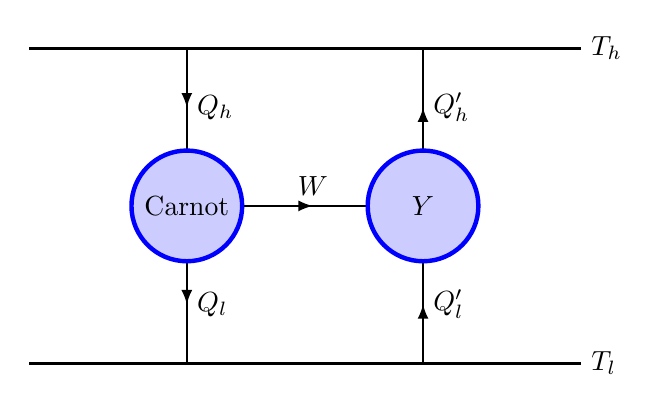
\begin{tikzpicture}
    \begin{scope}[thick, decoration={
    markings,
    mark=at position 0.5 with {\arrow{>}}}
    ] 
        \draw[very thick, black] (0, 0) -- (7, 0) node[right] {$T_l$};
        \draw[very thick, black] (0, 4) -- (7, 4) node[right] {$T_h$};
        
        \draw[postaction={decorate}] (2,1.5)-- node [right] {$Q_l$} (2,0) ;
        \draw[postaction={decorate}] (2,4)-- node [right] {$Q_h$} (2,2.5);
        \draw[postaction={decorate}] (2.5, 2) --node[above] {$W$} (4.7, 2) ;
        \draw[] (2, 2) node [fill = blue!20, draw = blue, ultra thick, circle, minimum size=4em] {Carnot};

        \draw[postaction={decorate}] (5,0)-- node [right] {$Q_l'$} (5,1.5) ;
        \draw[postaction={decorate}] (5,2.5)-- node [right] {$Q_h'$} (5,4);
        \draw[] (5, 2) node [fill = blue!20, draw = blue, ultra thick, circle, minimum size=4em] {$Y$};
    \end{scope}
\end{tikzpicture}

\end{document}